
\section{McSat: An extension of SMT Solvers}

\subsection{Introduction}


Mcsat is an extension of usual SMT solvers, introduced in~\cite{VMCAI13} and~\cite{FMCAD13}.
In usual SMT Solvers, interaction betweenthe core SAT Solver and the Theory is pretty limited~:
the SAT Solver make boolean decision, and sends them to the theory, whose role is inr eturn to
stop the SAT Solver as soons as the current set of assumptions is incoherent. This means
that the information that theories can give the SAT Solver is pretty limited, furthermore
it limits the ability of theories to guide the proof search.

While it appears to leave a reasonably simple job to the theory, since it completely
hides the propositional structure of the problem, this simple interaction between the
SAT Solver and the theory makes it harder to combine multiple theories into one.

McSat extends the SAT paradigm by allowing more exchange of information between the theory
and the SAT Solver. For instance, if the SAT Solver assumes a formula $x = 0$,
an arithmetic theory could propagate to the SAT Solver that the formula $x < 1$ must also hold,
instead of waiting for the SAT Solver to guess the truth value of $x < 1$ and possibly
inform the SAT Solver that the conjunction~: $x = 0 \land \neg x < 1$ is incoherent.

This exchange of information between the SAT Solver and the theories is done
by constructing a model throughout the proof search (which explains the name
Model Constructing SAT). This is achieved by extending the SAT Solver to not only
decide on boolean value of propositions, but to also decide on assignment of values
to expressions that appear in the problem.

\subsection{SMT Solver architecture}

We can represent a simplified version of the information flow (not taking into
account backtracking) of SMT Solvers, using the graph in fig~\ref{fig:smt_flow}.
In a pure Sat solver, the solver starts by doing
boolean propagation until no more literal can be propagated, at which point it
makes a decision and assign a truth value to a literal not yet assigned. It then
loops to its starting point and does boolean propagation. In an Smt solver,
after each boolean propagation, the solver sends the newly assigned literals
to the theory. The theory can then declare the current set of literals incoherent,
and give the solver a tautology which evaluates to $\bot$ in the current
(boolean) assignment.

\begin{figure}
  \begin{center}
    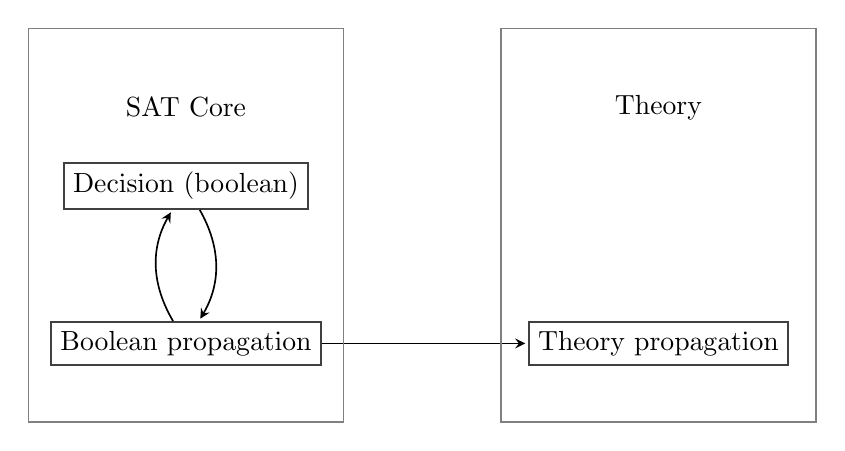
\begin{tikzpicture}[
        ->, % Arrow style
        > = stealth, % arrow head style
        shorten > = 1pt, % don't touch arrow head to node
        node distance = 2cm, % distance between nodes
        semithick, % line style
        auto
      ]

      \tikzstyle{state}=[rectangle,draw=black!75]

      \node (sat) {SAT Core};
      \node (th) [right of=sat, node distance=6cm] {Theory};
      \node[state] (d) [below of=sat, node distance=1cm] {Decision (boolean)};
      \node[state] (bp) [below of=d, node distance=2cm] {Boolean propagation};
      \node[state] (tp) [right of=bp, node distance=6cm] {Theory propagation};

      \path (d) edge [bend left=30] (bp);
      \path (bp) edge [bend left=30] (d);
      \path (bp) edge (tp);

      \draw[black!50] (-2,1) rectangle (2,-4);
      \draw[black!50] (4,1) rectangle (8,-4);

    \end{tikzpicture}
  \end{center}
  \caption{Simplified SMT Solver architecture}\label{fig:smt_flow}
\end{figure}

The main addition of McSat is that when the solver makes a decision, instead of
being restricted to making boolean assignment of formulas, the solver now can
decide to assign a term belonging to one of the literals. In order to do so,
the solver first chooses a term that has not yet been assigned, and then asks
the theory for a possible assignment. Like in usual SMT Solvers, a McSat solver
only exchange information with one theory, but, as we will see, combination
of theories become easier.

Since terms have assignments, the theory can now do useful and efficient
propagation of formulas implied by the current assignments.
The information flow then looks like fig~\ref{fig:mcsat_flow}.
For a more detailed presentation, see~\cite{FMCAD13} and~\cite{VMCAI13}.

\begin{figure}
  \begin{center}
    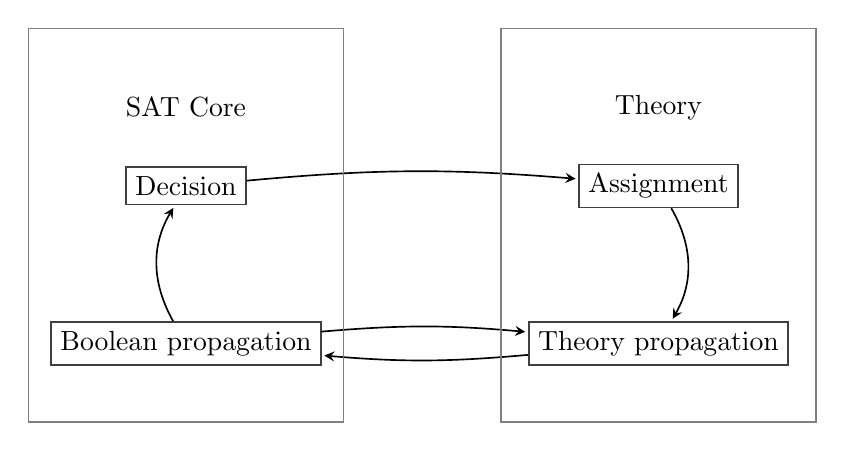
\begin{tikzpicture}[
        ->, % Arrow style
        > = stealth, % arrow head style
        shorten > = 1pt, % don't touch arrow head to node
        node distance = 2cm, % distance between nodes
        semithick, % line style
        auto
      ]

      \tikzstyle{state}=[rectangle,draw=black!75]

      \node (sat) {SAT Core};
      \node (th) [right of=sat, node distance=6cm] {Theory};
      \node[state] (d) [below of=sat, node distance=1cm] {Decision};
      \node[state] (ass) [right of=d, node distance=6cm] {Assignment};
      \node[state] (bp) [below of=d, node distance=2cm] {Boolean propagation};
      \node[state] (tp) [right of=bp, node distance=6cm] {Theory propagation};

      \path (bp)[right] edge [bend left=5] (tp);
      \path (tp) edge [bend left=5] (bp);
      \path (bp) edge [bend left=30] (d);
      \path (d) edge [bend left=5] (ass);
      \path (ass) edge [bend left=30] (tp);

      \draw[black!50] (-2,1) rectangle (2,-4);
      \draw[black!50] (4,1) rectangle (8,-4);

    \end{tikzpicture}
  \end{center}
  \caption{Simplified McSat Solver architecture}\label{fig:mcsat_flow}
\end{figure}

\subsection{Expected theory invariants}

We write $\mathbb{E}$ for the (infinite) set of first-order expressions,
and $\mathbb{F}$ for the set of formulas.

During proof search are maintained a set of assertions $\mathcal{S}$
and a partial assignment $\sigma$ as a involution of $\mathbb{E} \cup \mathbb{F}$,
with only a finite number of $x \in \mathbb{E} \cup \mathbb{F}$ such that $\sigma(x) \neq x$.
We say that $\mathcal{S}$ is coherent with $\sigma$ iff for every $\varphi \in \mathcal{S}$,
$\varphi\sigma$ is satisfiable (independently from the rest of the formulas in $\mathcal{S}$).
Intuitively, this represents the fact that the substitution $\sigma$ does not imply
ground contradictions.

A theory then has to ensure that for every expression $e \in \mathbb{E} \cup \mathbb{F}$,
there exists $v \in \mathbb{E} \cup \mathbb{F}$ such that $\mathcal{S}$ is coherent with
$\sigma \cup \{ e \rightarrow v \}$\footnote{Note that in particular, this implies
that $\mathcal{S}$ is coherent with $\sigma$}. As soon as that is not the case, the theory
should inform the SAT Solver to backtrack, since the current branch is clearly not satisfiable.

